% answers.tex —— 1977 年·江苏南通卷 · 参考答案与详细解析片段
% 由 tools/generate_projects.py 依来源总账自 1977/1977_数学真题_江苏南通_试题.md + 1977/1977_数学真题_江苏南通_解析正文.md + 1977/1977_数学真题_江苏南通_答案要点.md 生成，勿手改（改源 MD 后重跑）


\begin{gktip}
固定源是题面与解答连续排印的书籍扫描（书籍页码 118—122）。下文逐题独立推导，并与源解答对照复核。两处源卷排印问题预告：第 9 题源解答对角线一步的根号内多印一项平方项（见该题源注），第 10 题源解答首个比例式分母在 β 前多印一个角符号（见该题源注）；两处均按数学上自洽的方式理解，不影响最终结论。
\end{gktip}

\begin{answer}
\gksolhead{1}{}

\textbf{题目}（10 分）：

回答下列问题：

（1） 当 $a$ 为何值时，$2a>a$；当 $a$ 为何值时，$2a=a$；当 $a$ 为何值时 $2a<a$。

（2） 当 $x$ 为何值时，$|x|=x$。

\Needspace{4\baselineskip}
\textbf{解析}

\gksubpart{（1）}

三组比较都可归结为差 $2a-a=a$ 的符号：

\begin{itemize}
\item 当 $a>0$ 时差为正，所以 $2a>a$；
\item 当 $a=0$ 时 $2a=0=a$；
\item 当 $a<0$ 时差为负，所以 $2a<a$。
\end{itemize}

\gksubpart{（2）}

按绝对值的定义：$x\ge 0$ 时 $|x|=x$；$x<0$ 时 $|x|=-x>0>x$，此时 $|x|\ne x$。因此使 $|x|=x$ 成立的是 $x\ge 0$（含 $x=0$）。

\gkanswer{答案（1）：$a>0$ 时 $2a>a$；$a=0$ 时 $2a=a$；$a<0$ 时 $2a<a$。}

\gkanswer{答案（2）：$x\ge 0$。}

\end{answer}
\begin{answer}
\gksolhead{2}{}

\textbf{题目}（10 分）：

写出下列函数的自变量 $x$ 的取值范围（在实数范围内）；

（1） $y=\dfrac{1}{2-x}$

（2） $y=\sqrt{2x-1}$

\Needspace{4\baselineskip}
\textbf{解析}

\gksubpart{（1）}

分母不能为零：$2-x\ne 0$，即 $x\ne 2$。所以函数 $y=\dfrac{1}{2-x}$ 的自变量取值范围是 $x\ne 2$。

\gksubpart{（2）}

二次根号内须非负：$2x-1\ge 0$，即 $x\ge\dfrac{1}{2}$。所以函数 $y=\sqrt{2x-1}$ 的自变量取值范围是 $x\ge\dfrac{1}{2}$。

\gkanswer{答案（1）：$x\ne 2$。}

\gkanswer{答案（2）：$x\ge\dfrac{1}{2}$。}

\end{answer}
\begin{answer}
\gksolhead{3}{}

\textbf{题目}（10 分）：

\Needspace{5\baselineskip}
计算

\nopagebreak[4]
\[
\left(\frac{2}{3}\right)^{2}+(-5.8)^{0}-\left(\frac{8}{27}\right)^{-\frac{2}{3}}+\left(\frac{1}{2}\right)^{-2}.
\]

\Needspace{4\baselineskip}
\textbf{解析}

逐项化简：$\left(\dfrac{2}{3}\right)^{2}=\dfrac{4}{9}$；$(-5.8)^{0}=1$；$\dfrac{8}{27}=\left(\dfrac{2}{3}\right)^{3}$，故 $\left(\dfrac{8}{27}\right)^{-\frac{2}{3}}=\left(\dfrac{2}{3}\right)^{-2}=\dfrac{9}{4}$；$\left(\dfrac{1}{2}\right)^{-2}=4$。

\Needspace{5\baselineskip}
于是

\nopagebreak[4]
\[
\frac{4}{9}+1-\frac{9}{4}+4
=\frac{16+36-81+144}{36}
=\frac{115}{36}=3\frac{7}{36}.
\]

\gkanswer{答案：$3\dfrac{7}{36}$（即 $\dfrac{115}{36}$）。}

\end{answer}
\begin{answer}
\gksolhead{4}{}

\textbf{题目}（10 分）：

$k$ 为何值时，方程 $x^{2}-2kx+4=0$ 有两个相等的实数根？并求出这方程的根。

\Needspace{4\baselineskip}
\textbf{解析}

\Needspace{5\baselineskip}
判别式

\nopagebreak[4]
\[
\Delta=(-2k)^{2}-4\times 4=4k^{2}-16.
\]

方程有两个相等的实数根当且仅当 $\Delta=0$，即 $4k^{2}-16=0$，得 $k=\pm 2$。

$k=2$ 时，原方程为 $x^{2}-4x+4=0$，即 $(x-2)^{2}=0$，两相等实数根为 $x_1=x_2=2$；

$k=-2$ 时，原方程为 $x^{2}+4x+4=0$，即 $(x+2)^{2}=0$，两相等实数根为 $x_1=x_2=-2$。

\gkanswer{答案：$k=\pm 2$；$k=2$ 时两相等实数根为 $x_1=x_2=2$，$k=-2$ 时两相等实数根为 $x_1=x_2=-2$。}

\end{answer}
\begin{answer}
\gksolhead{5}{}

\textbf{题目}（10 分）：

已知 $\sin\alpha=\dfrac{3}{5}$（$90^\circ<\alpha<180^\circ$），求 $\cos\alpha$，$\operatorname{tg}\alpha$，$\operatorname{ctg}\alpha$。

\Needspace{4\baselineskip}
\textbf{解析}

\Needspace{5\baselineskip}
因 $90^\circ<\alpha<180^\circ$，$\alpha$ 在第二象限，$\cos\alpha<0$，故

\nopagebreak[4]
\[
\cos\alpha=-\sqrt{1-\sin^{2}\alpha}
=-\sqrt{1-\frac{9}{25}}
=-\sqrt{\frac{16}{25}}=-\frac{4}{5}.
\]

\nopagebreak[4]
\[
\operatorname{tg}\alpha=\frac{\sin\alpha}{\cos\alpha}
=\frac{\frac{3}{5}}{-\frac{4}{5}}=-\frac{3}{4},
\qquad
\operatorname{ctg}\alpha=\frac{1}{\operatorname{tg}\alpha}=-\frac{4}{3}=-1\frac{1}{3}.
\]

\gkanswer{答案：$\cos\alpha=-\dfrac{4}{5}$，$\operatorname{tg}\alpha=-\dfrac{3}{4}$，$\operatorname{ctg}\alpha=-\dfrac{4}{3}$（即 $-1\dfrac{1}{3}$）。}

\end{answer}
\begin{answer}
\gksolhead{6}{}

\textbf{题目}（10 分）：

试写出抛物线 $y=1+4x-2x^{2}$ 的顶点坐标，对称轴方程和函数 $y$ 的极值。

\Needspace{4\baselineskip}
\textbf{解析}

\Needspace{5\baselineskip}
配方：

\nopagebreak[4]
\[
\begin{aligned}
y&=1+4x-2x^{2}
=-2\left(x^{2}-2x-\frac{1}{2}\right)
=-2\left[(x-1)^{2}-\frac{3}{2}\right]\\
&=-2(x-1)^{2}+3.
\end{aligned}
\]

所以顶点坐标为 $(1,3)$，对称轴方程为 $x=1$。因 $a=-2<0$，抛物线开口向下，函数 $y$ 有最大值：当 $x=1$ 时，$y_{\text{\text{最大}}}=3$。

（源解答另用 $x=-\dfrac{b}{2a}$ 与 $\dfrac{4ac-b^{2}}{4a}$ 验证，结果一致。）

\gkanswer{答案：顶点坐标 $(1,3)$，对称轴方程 $x=1$，函数 $y$ 有最大值 $3$。}

\end{answer}
\begin{answer}
\gksolhead{7}{}

\textbf{题目}（10 分）：

\Needspace{5\baselineskip}
解方程

\nopagebreak[4]
\[
\frac{\lg 2x}{\lg (x-4)}=2.
\]

\Needspace{4\baselineskip}
\textbf{解析}

方程有意义要求真数为正且底不为 $1$：$x-4>0$ 且 $x-4\ne 1$，即 $x>4$ 且 $x\ne 5$。

\Needspace{5\baselineskip}
由 $\dfrac{\lg 2x}{\lg (x-4)}=2$ 得 $\lg 2x=2\lg (x-4)=\lg (x-4)^{2}$，于是

\nopagebreak[4]
\[
2x=(x-4)^{2},
\qquad
x^{2}-10x+16=0,
\qquad
(x-8)(x-2)=0.
\]

$x=8$：满足 $x>4$ 且 $x\ne 5$，代回原式 $\dfrac{\lg 16}{\lg 4}=\dfrac{2\lg 4}{\lg 4}=2$，是原方程的根；

$x=2$：使 $x-4<0$，破坏定义域，是增根，应舍去。

\gkanswer{答案：$x=8$；$x=2$ 是增根，应舍去。}

\end{answer}
\begin{answer}
\gksolhead{8}{}

\textbf{题目}（10 分）：

求 $200$ 以内的能被 $6$ 整除的所有自然数的和。

\Needspace{4\baselineskip}
\textbf{解析}

\Needspace{5\baselineskip}
$200$ 以内能被 $6$ 整除的自然数为 $6,12,\cdots,198$。由 $200=33\times 6+2$ 知共 $33$ 项，它是首项为 $6$、末项为 $198$ 的等差数列，其和为

\nopagebreak[4]
\[
S=6\times(1+2+\cdots+33)
=6\times\frac{33\times 34}{2}
=3366.
\]

源解答按 $S_{33}=\dfrac{33}{2}\times\left(6+6\times 33\right)=\dfrac{33}{2}\times 204=3366$ 计算，结果一致。

\gkanswer{答案：$3366$。}

\end{answer}
\begin{answer}
\gksolhead{9}{}

\textbf{题目}（10 分）：

已知正四棱锥底面边长为 $12\,\mathrm{cm}$，高为 $2\sqrt{7}\ \mathrm{cm}$，求它的侧棱。

\begin{gktip}
原源 PDF 第 5 页附有正四棱锥及其高、底面对角线的示意图；LaTeX 版按源图重绘。
\end{gktip}
\nopagebreak[4]
\begin{center}% 1977 年江苏南通卷第九题：正四棱锥 P-ABCD（P 顶点、O 底面中心），
% 高 PO 与底面对角线 AC 为虚线（按源卷第 5 页布局）
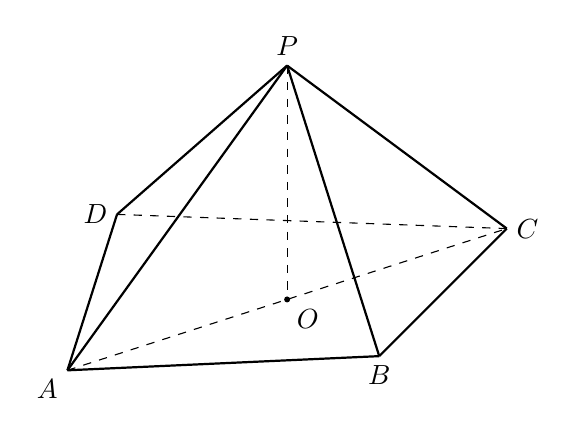
\begin{tikzpicture}[scale=0.9]
  \coordinate (A) at (0,0);
  \coordinate (B) at (4.4,0.2);
  \coordinate (C) at (6.2,2.0);
  \coordinate (D) at (0.7,2.2);
  \coordinate (P) at (3.1,4.3);
  \coordinate (O) at (3.1,1.0);
  \draw[thick] (P)--(A);
  \draw[thick] (P)--(B);
  \draw[thick] (P)--(C);
  \draw[thick] (P)--(D);
  \draw[thick] (A)--(B);
  \draw[thick] (B)--(C);
  \draw[thick] (D)--(A);
  \draw[dashed] (D)--(C);
  \draw[dashed] (A)--(C);
  \draw[dashed] (P)--(O);
  \fill (O) circle (1.2pt) node[below right] {$O$};
  \node[above] at (P) {$P$};
  \node[below left] at (A) {$A$};
  \node[below] at (B) {$B$};
  \node[right] at (C) {$C$};
  \node[left] at (D) {$D$};
\end{tikzpicture}
\end{center}
\nopagebreak[4]
\Needspace{4\baselineskip}
\textbf{解析}

如图，正四棱锥 $P-ABCD$ 的高 $PO=2\sqrt{7}\ \mathrm{cm}$，底面正方形边长 $AB=BC=12\ \mathrm{cm}$。
\nopagebreak[4]
\begin{center}% 1977 年江苏南通卷第九题：正四棱锥 P-ABCD（P 顶点、O 底面中心），
% 高 PO 与底面对角线 AC 为虚线（按源卷第 5 页布局）
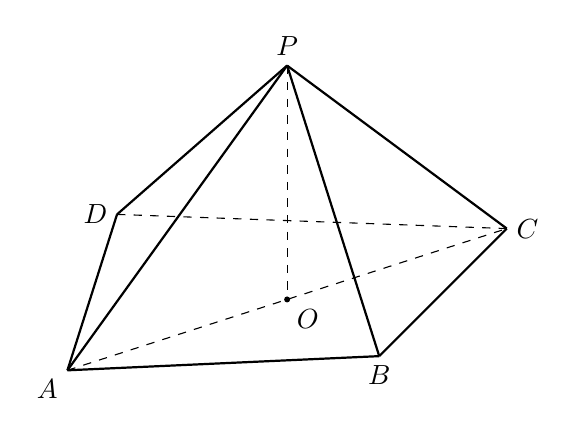
\begin{tikzpicture}[scale=0.9]
  \coordinate (A) at (0,0);
  \coordinate (B) at (4.4,0.2);
  \coordinate (C) at (6.2,2.0);
  \coordinate (D) at (0.7,2.2);
  \coordinate (P) at (3.1,4.3);
  \coordinate (O) at (3.1,1.0);
  \draw[thick] (P)--(A);
  \draw[thick] (P)--(B);
  \draw[thick] (P)--(C);
  \draw[thick] (P)--(D);
  \draw[thick] (A)--(B);
  \draw[thick] (B)--(C);
  \draw[thick] (D)--(A);
  \draw[dashed] (D)--(C);
  \draw[dashed] (A)--(C);
  \draw[dashed] (P)--(O);
  \fill (O) circle (1.2pt) node[below right] {$O$};
  \node[above] at (P) {$P$};
  \node[below left] at (A) {$A$};
  \node[below] at (B) {$B$};
  \node[right] at (C) {$C$};
  \node[left] at (D) {$D$};
\end{tikzpicture}
\end{center}
\nopagebreak[4]
\Needspace{5\baselineskip}
底面正方形的对角线

\nopagebreak[4]
\[
AC=\sqrt{AB^{2}+BC^{2}}=\sqrt{12^{2}+12^{2}}=12\sqrt{2}\ (\mathrm{cm}),
\qquad
AO=\frac{AC}{2}=6\sqrt{2}\ (\mathrm{cm}).
\]

\Needspace{5\baselineskip}
侧棱

\nopagebreak[4]
\[
\begin{aligned}
PA&=\sqrt{PO^{2}+AO^{2}}
=\sqrt{\left(2\sqrt{7}\right)^{2}+\left(6\sqrt{2}\right)^{2}}\\
&=\sqrt{28+72}=\sqrt{100}=10\ (\mathrm{cm}).
\end{aligned}
\]

即侧棱长为 $10\ \mathrm{cm}$。

\begin{gktip}
\textbf{源注}：源解答在对角线一步的根号内多印一项平方项（印作两个 12 的平方之外再加一个 2 的平方字样），而紧随其后的结果直接写 12 倍根号 2；按前式应只为基础边长平方之和，本文按不含该项计算，结果不变。
\end{gktip}

\gkanswer{答案：侧棱长为 $10\ \mathrm{cm}$。}

\end{answer}
\begin{answer}
\gksolhead{10}{}

\textbf{题目}（10 分）：

两根钢绳悬吊货物时，两条钢绳与铅垂线的夹角分别为 $\alpha$ 和 $\beta$，货物的重量为 $P$，试用表达式分别写出钢绳所承受的拉力 $F_1$ 和 $F_2$

\begin{gktip}
原源 PDF 第 5 页附有两条钢绳拉力与重力的受力示意图（图上编有 1、2、3、4 号角）；LaTeX 版按源图重绘。
\end{gktip}
\nopagebreak[4]
\begin{center}% 1977 年江苏南通卷第十题：两根钢绳悬吊货物的受力示意（按源卷第 5 页布局）：
% 结点处 F1（左上）、F2（右上）两条拉力与竖直向下重力 P，上方虚线把 F1、F2
% 作用线延长到竖直线交成力三角形，1、2 号角在结点处，3 号角在顶点处，4 号角在 F1 箭头端处
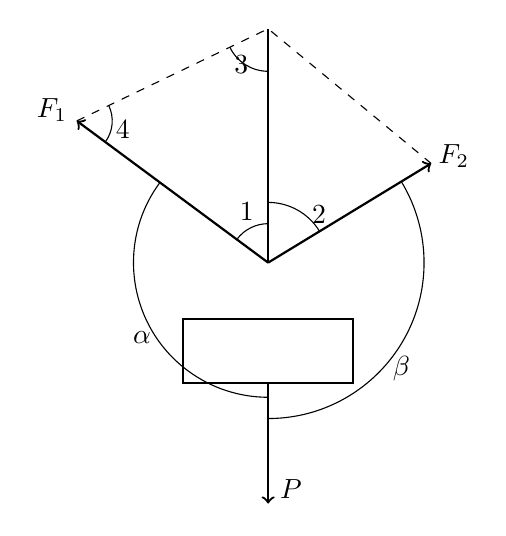
\begin{tikzpicture}[scale=0.9]
  \coordinate (K) at (0,0);
  \coordinate (T) at (0,3.3);
  \coordinate (L) at (-2.7,2.0);
  \coordinate (R) at (2.3,1.4);
  \draw[thick,->] (0,0)--(L);
  \node at (-3.05,2.15) {$F_1$};
  \draw[thick,->] (0,0)--(R);
  \node at (2.62,1.5) {$F_2$};
  \draw[thick] (0,0)--(T);
  \draw[dashed] (L)--(T);
  \draw[dashed] (R)--(T);
  \draw[thick] (-1.2,-0.8) rectangle (1.2,-1.7);
  \draw[thick,->] (0,-1.7)--(0,-3.4);
  \node at (0.32,-3.2) {$P$};
  \draw (90:0.55) arc[start angle=90, end angle=143.5, radius=0.55];
  \node at (-0.3,0.72) {$1$};
  \draw (90:0.85) arc[start angle=90, end angle=31.3, radius=0.85];
  \node at (0.72,0.68) {$2$};
  \begin{scope}[shift={(0,3.3)}]
    \draw (205.7:0.6) arc[start angle=205.7, end angle=270, radius=0.6];
  \end{scope}
  \node at (-0.38,2.8) {$3$};
  \begin{scope}[shift={(-2.7,2.0)}]
    \draw (25.7:0.5) arc[start angle=25.7, end angle=-36.5, radius=0.5];
  \end{scope}
  \node at (-2.05,1.88) {$4$};
  \draw (143.5:1.9) arc[start angle=143.5, end angle=270, radius=1.9];
  \node at (-1.78,-1.05) {$\alpha$};
  \draw (270:2.2) arc[start angle=270, end angle=391.3, radius=2.2];
  \node at (1.88,-1.5) {$\beta$};
\end{tikzpicture}
\end{center}
\nopagebreak[4]
\Needspace{4\baselineskip}
\textbf{解析}

如图，结点处受三个力：两根钢绳的拉力 $F_1$、$F_2$（与铅垂线的夹角分别为 $\alpha$、$\beta$）和竖直向下的重力 $P$。
\nopagebreak[4]
\begin{center}% 1977 年江苏南通卷第十题：两根钢绳悬吊货物的受力示意（按源卷第 5 页布局）：
% 结点处 F1（左上）、F2（右上）两条拉力与竖直向下重力 P，上方虚线把 F1、F2
% 作用线延长到竖直线交成力三角形，1、2 号角在结点处，3 号角在顶点处，4 号角在 F1 箭头端处
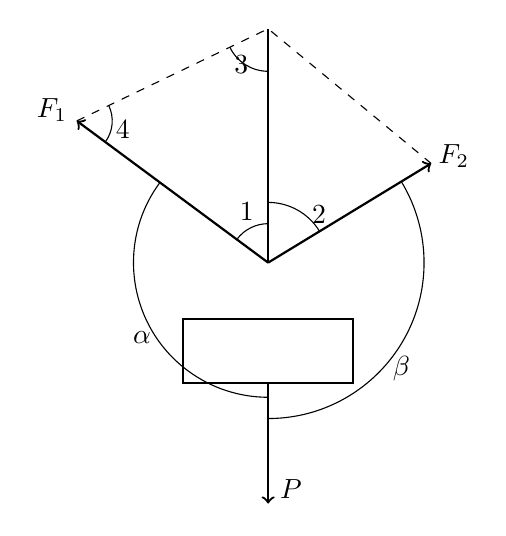
\begin{tikzpicture}[scale=0.9]
  \coordinate (K) at (0,0);
  \coordinate (T) at (0,3.3);
  \coordinate (L) at (-2.7,2.0);
  \coordinate (R) at (2.3,1.4);
  \draw[thick,->] (0,0)--(L);
  \node at (-3.05,2.15) {$F_1$};
  \draw[thick,->] (0,0)--(R);
  \node at (2.62,1.5) {$F_2$};
  \draw[thick] (0,0)--(T);
  \draw[dashed] (L)--(T);
  \draw[dashed] (R)--(T);
  \draw[thick] (-1.2,-0.8) rectangle (1.2,-1.7);
  \draw[thick,->] (0,-1.7)--(0,-3.4);
  \node at (0.32,-3.2) {$P$};
  \draw (90:0.55) arc[start angle=90, end angle=143.5, radius=0.55];
  \node at (-0.3,0.72) {$1$};
  \draw (90:0.85) arc[start angle=90, end angle=31.3, radius=0.85];
  \node at (0.72,0.68) {$2$};
  \begin{scope}[shift={(0,3.3)}]
    \draw (205.7:0.6) arc[start angle=205.7, end angle=270, radius=0.6];
  \end{scope}
  \node at (-0.38,2.8) {$3$};
  \begin{scope}[shift={(-2.7,2.0)}]
    \draw (25.7:0.5) arc[start angle=25.7, end angle=-36.5, radius=0.5];
  \end{scope}
  \node at (-2.05,1.88) {$4$};
  \draw (143.5:1.9) arc[start angle=143.5, end angle=270, radius=1.9];
  \node at (-1.78,-1.05) {$\alpha$};
  \draw (270:2.2) arc[start angle=270, end angle=391.3, radius=2.2];
  \node at (1.88,-1.5) {$\beta$};
\end{tikzpicture}
\end{center}
\nopagebreak[4]
\Needspace{5\baselineskip}
三力平衡，$F_1$、$F_2$ 与 $P$ 构成封闭的力三角形。$F_1$ 与 $F_2$ 方向的夹角为 $\alpha+\beta$，故力三角形中 $P$ 边所对的角为 $180^\circ-(\alpha+\beta)$；$F_1$ 边所对的角是 $F_2$ 与 $P$ 方向的夹角 $180^\circ-\beta$。由正弦定理，

\nopagebreak[4]
\[
\frac{F_1}{\sin(180^\circ-\beta)}
=\frac{P}{\sin\bigl[180^\circ-(\alpha+\beta)\bigr]},
\]

\Needspace{5\baselineskip}
所以

\nopagebreak[4]
\[
F_1=\frac{P\sin(180^\circ-\beta)}{\sin\bigl[180^\circ-(\alpha+\beta)\bigr]}
=\frac{P\sin\beta}{\sin(\alpha+\beta)}.
\]

\Needspace{5\baselineskip}
同理

\nopagebreak[4]
\[
F_2=\frac{P\sin\alpha}{\sin(\alpha+\beta)}.
\]

特例校验：当 $\alpha=\beta$ 时，$F_1=F_2=\dfrac{P}{2\cos\alpha}$，与对称吊挂时两绳各承担一半重力的水平分量为零、合力沿竖直方向的直觉相符。

\begin{gktip}
\textbf{源注}：源解答先由图上编号角过渡（1、2 号角各为 $180^\circ$ 减 $\alpha$、减 $\beta$，3 号角与 2 号角相同），再写出比例式，其右端取 $-\dfrac{P}{\sin(\alpha+\beta-180^\circ)}$，左端分母在 $\beta$ 前多印一个角符号，系衍字。两式等价：$\sin(\alpha+\beta-180^\circ)=-\sin\bigl[180^\circ-(\alpha+\beta)\bigr]$。
\end{gktip}

\gkanswer{答案：$F_1=\dfrac{P\sin\beta}{\sin(\alpha+\beta)}$，$F_2=\dfrac{P\sin\alpha}{\sin(\alpha+\beta)}$。}

\end{answer}